\section[Critérios de Avaliação das Ferramentas]{Critérios de Avaliação das Ferramentas}
Sobre os critérios de qualidade definidos, avaliou-se:

\begin{itemize}
  \item Armazenamento dos requisitos e de seus atributos: nesses pontos, o foco da avaliação era descobrir a capacidade da ferramenta em guardar informações sobre os requisitos. Visto que há a possibilidade da mesma alterar ou simplesmente apagar dados inseridos, buscou-se via testes e manual da ferramenta descobrir se com o uso da mesma, estava-se livre de tal risco.

  \item Artefatos que estão relacionados: nessa avaliação, buscou-se compreender e definir quais as relações presentes em dado requisito, ou seja, se o mesmo se relaciona com outros requisitos e se ao fim de dada iteração, algum documento é gerado.

  \item Gestão de mudanças: buscou-se avaliar o comportamento da ferramenta no que diz respeito as mudanças que o requisito pode sofrer ao longo do projeto. A importância de se avaliar isso tange a questão da qualidade do que foi proposto, se de fato é pouco mutável e menos sucetível a falhas.

  \item Rastreabilidade dos requisitos: buscou-se a avaliação para saber se a rastreabilidade dos requisitos é realizada de maneira satisfatória, fornecendo características essenciais como requisitos que derivam do requisito em questão e requisitos que advêm o mesmo.

  \item Flexibilidade e usabilidade: com essa questão, buscou-se avaliar as facilidades encontradas no manuseio da ferramenta, se ela possuia nomes significativos, se a mesma é executada de maneira fluída, sem muitos travamentos, se a interface era fácil de se usar e se era fácil de se lembrar como se usa.

  \item Adaptação ao contexto: nesse ponto, fez-se uma verificação e análise a fim de descobrir se a ferramenta oferecia um suporte considerável e único para a abordagem definida pelo time e para o processo de Engenharia de Requisitos da Empresa Junior de Engenharia de Requisitos da Universidade de Brasília.
\end{itemize}

Após a pesquisa das ferramentas para gestão de requisitos e a analise de cada uma das encontradas, fizemos um quadro comparativo que avalia cada uma das ferramentas com os quesitos nele especificado. Cada um desses quesitos foram avaliados de 0 a 5, sendo:

0 - Muito ruim

1 - Ruim

2 - Razoável

3 - Bom

4 - Muito bom

5 - Excelente

O quadro comparativo ficou da seguinte maneira:
\begin{figure}[!htb]
\centering
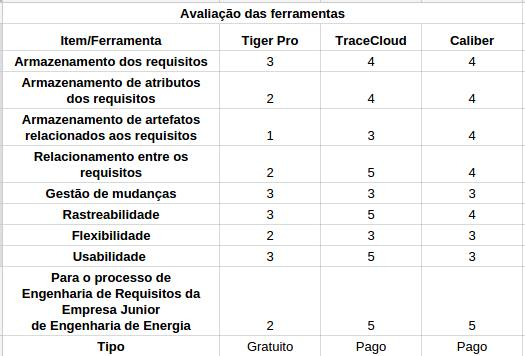
\includegraphics[scale=0.7]{figuras/quadro.jpg}
\caption{Quadro comparativo entre ferramentas}
\end{figure}


